\documentclass{./../../Latex/teaching_slides}

\usepackage{venndiagram}
\usepackage{tikz}
\usepackage{pgfplots}
\usetikzlibrary{arrows.meta}

\begin{document}

\title{ECON 441 \\ \vspace{0.4em} \normalsize Introduction to Mathematical Economics}
\author{Div Bhagia}
\date{Lecture 11 \\~\\ Envelope Theorem, Quasiconcavity, \\
Convex sets, Homogenous Functions}

%%%%%%%%%%%%%%
\begin{frame}[noframenumbering, plain]
\maketitle
\end{frame}

%%%%%%%%%%%%%%
\begin{frame}{Profit Maximization}
Maximize:
$$ \pi(L) = AL^{\alpha}-wL, \quad \quad 0 < \alpha <1 $$ \\~\\

First-order condition:
$$ \pi'(L) = \alpha A L^{\alpha-1}-w = 0 \rightarrow L^* = \left(\frac{\alpha A}{w}\right)^{\frac{1}{1-\alpha}} $$


Optimal labor input is a function of wages, we can write $L^*(w)$. \\~\\
Also, we wrote $\pi()$ as a function of $L$, but it also depends on $w$ (and $\alpha$) which are \textit{exogenous} parameters.
\end{frame}

%%%%%%%%%%%%%%
\begin{frame}{Profit Maximization}
We are often interested in questions like: \\
\begin{itemize}
  \item[] How does the profit change due to change in wages? \\~\\
\end{itemize}
Remember, $$ \pi(L) = A L^{\alpha}-wL$$
So optimal profit depends directly on $w$ but also indirectly through $L$
\end{frame}


%%%%%%%%%%%%%%
\begin{frame}{Maximum Value Function}
Maximum value function: objective function after plugging in optimal values for the choice \textit{variables} \\~\\

Maximum value function is a function of \textit{parameters} \\~\\
For the profit maximization problem, the value function:
\begin{align*}
	 V(w) = \pi(L^*(w), w) &= A L^*(w)^{\alpha}-wL^*(w) 
\end{align*}
Plugging in $L^*(w) = \left(\frac{A \alpha}{w}\right)^{\frac{1}{1-\alpha}}$, we get:
$$ V(w)  = A\left(\frac{\alpha A}{w}\right)^{\frac{\alpha}{1-\alpha}}-w \left(\frac{\alpha A}{w}\right)^{\frac{1}{1-\alpha}} $$


\end{frame}

%%%%%%%%%%%%%%
\begin{frame}{Profit Maximization}
Value function:
\begin{align*}
	 V(w) = \pi^* = \pi(L^*(w), w) \\
\end{align*}
To see how optimal profit $V(w)$ changes with wages:
$$ V'(w) = \underbrace{\pi^*_{L} \cdot \frac{d L^*}{d w}}_{\textit{Indirect Effect}} + \underbrace{\pi^*_{w}}_{\textit{Direct Effect}}$$
\pause But by the F.O.C, $\pi^*_{L} =0$, so
$$ V'(w) = \pi^*_{w} $$
\end{frame}

%%%%%%%%%%%%%%
\begin{frame}{Envelope Theorem}
$$ V'(w) = \pi^*_{w} $$
\vspace{0.25em}

This result says that at the optimum, as wages vary, with labor allowed to
adjust optimally gives the same result as if labor was held fixed. \\~\\

In other words, only the direct effect of wages matters, even though it enters indirectly through choice of labor input as well. \\~\\

This is actually a general result called the \textit{envelope theorem}.

\end{frame}

%%%%%%%%%%%%%%
\begin{frame}{Profit Maximization}
How does the profit change due to a change in wages?
$$ \pi^* = AL^*(w)^{\alpha}-wL^*(w) $$

The answer is given by:
$$ \pi^*_w = -L^*(w) = - \left(\frac{\alpha A}{w}\right)^{\frac{1}{1-\alpha}} $$
Note that you would get the same answer by calculating $V'(w)$ using the expression on slide 3, but the envelope theorem suggests the above shortcut. 
\end{frame}

%%%%%%%%%%%%%%%%%%%%
\begin{frame}{Envelope Theorem}
\begin{center}
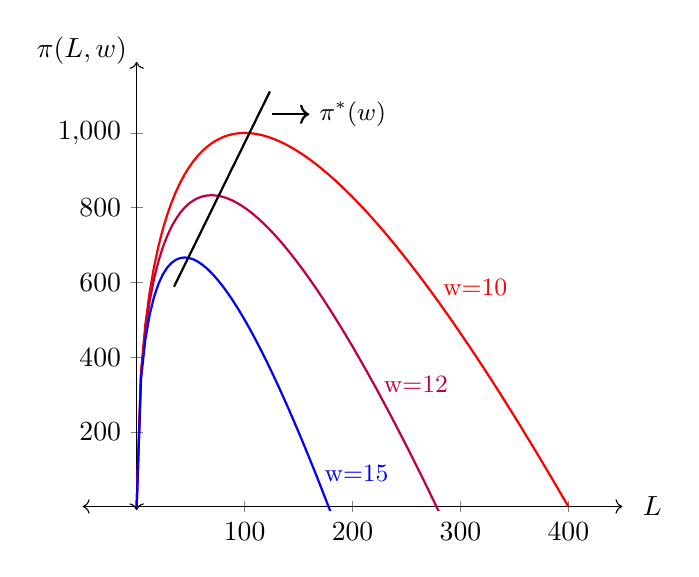
\begin{tikzpicture}
\begin{axis}[
    xlabel={$L$},
    ylabel={$\pi(L,w)$},
    samples=100,
    ymin=-10, ymax=1190,
    xmin=-50, xmax=450,
    axis lines=middle,
    axis line style=<->,
    ticklabel style={fill=white},
    every axis y label/.style={at={(ticklabel* cs:1.025)},anchor=east},
    every axis x label/.style={at={(ticklabel* cs:1.02)},anchor=west},
]

\def\A{200} % Define A
\def\alpha{0.5} % Define alpha
\addplot[red,  thick, domain=0:400] {\A*x^\alpha - 10*x};
\node[red, anchor=north west] at (axis cs:275,635){\small w=10};
\addplot[purple,  thick, domain=0:400] {\A*x^\alpha - 12*x};
\node[purple, anchor=north west] at (axis cs:220,375){\small w=12};
\addplot[blue,  thick, domain=0:400] {\A*x^\alpha - 15*x};
\node[blue, anchor=north west] at (axis cs:165,135){\small w=15};
\pgfmathsetmacro{\optLlow}{(\A*\alpha/9)^(1/(1-\alpha))}
\pgfmathsetmacro{\optLhigh}{(\A*\alpha/17)^(1/(1-\alpha))}
\draw [black, thick] (axis cs:\optLlow,\A*\optLlow^\alpha - 9*\optLlow) -- (axis cs:\optLhigh,\A*\optLhigh^\alpha - 17*\optLhigh);
\draw [->, black, thick] (axis cs:125,1050) -- (axis cs:160,1050) node[pos=1,anchor=west] {\small $\pi^*(w)$ }; ;

\end{axis}
\end{tikzpicture}
\end{center}
\end{frame}


%%%%%%%%%%%%%%
\begin{frame}{Envelope Theorem}
More generally, consider the following maximization problem with two choice variables $x$ and $y$, and one parameter, $\alpha$: \\~\\

Maximize
$$
U=f(x, y, \alpha) 
$$

\vspace{0.5em}
The first order necessary conditions are
$$
f_{x}(x, y, \alpha)=f_{y}(x, y, \alpha)=0
$$

\vspace{0.5em}
If the second-order conditions are met, these two equations implicitly define the solutions $x=x^{*}(\alpha) \quad y=x^{*}(\alpha)$.
\end{frame}

%%%%%%%%%%%%%%
\begin{frame}{Envelope Theorem}
If we substitute these solutions into the objective function, we obtain a new function:
$$
V(\alpha)=f\left(x^{*}(\alpha), y^{*}(\alpha), \alpha\right)
$$

\vspace{0.5em}
If we differentiate $V$ with respect to $\alpha$:
$$
\frac{d V}{d \alpha}=f_{x} \frac{\partial x^{*}}{\partial \alpha}+f_{y} \frac{\partial y^{*}}{\partial \alpha}+f_{\alpha}
$$

\vspace{0.5em}
From the first order conditions we know $f_{x}=f_{y}=0$, therefore
$$
\frac{d V}{d \alpha}=f_{\alpha}
$$
\end{frame}

%%%%%%%%%%%%%%
\begin{frame}{Envelope Theorem with Constraints}
We have a similar envelope theorem for constrained optimization problems such as  \\~\\
\hspace{1em} Maximize $U=f(x, y ; \alpha)$ subject to $G(x, y ; \alpha)=0$ \\~\\
Lagrangian function:
$$
L=f(x, y ; \alpha)+\lambda G(x, y ; \alpha)
$$
\end{frame}

%%%%%%%%%%%%%%
\begin{frame}{Envelope Theorem with Constraints}
Lagrangian function:
$$
L=f(x, y ; \alpha)+\lambda G(x, y ; \alpha)
$$

First-order conditions:
$$
\begin{aligned}
&L_{x}=f_{x}+\lambda G_{x}=0 \\
&L_{y}=f_{y}+\lambda G_{y}=0 \\
&L_{\lambda}=G(x, y ; \alpha)=0
\end{aligned}
$$
Solving this system of equations gives us
$$
x=x^{*}(\alpha) \quad y=y^{*}(\alpha) \quad \lambda=\lambda^{*}(\alpha)
$$

\end{frame}


%%%%%%%%%%%%%%
\begin{frame}{Envelope Theorem with Constraints}
Substituting the solutions into the objective function, we get
$$
U^{*}=f\left(x^{*}(\alpha), y^{*}(\alpha), \alpha\right)=V(\alpha)
$$

\vspace{0.5em}
By envelope theorem:
$$
\frac{d V(\alpha)}{d \alpha}=\frac{\partial L^{*}}{\partial \alpha}
$$
\end{frame}

%%%%%%%%%%%%%%
\begin{frame}{Interpretation of the Lagrange Multiplier}
An application of the envelope theorem for constrained optimization gives us the interpretation of the Lagrange multiplier. \\~\\
Consider the following problem: \\~\\
\hspace{1em} Maximize $U=f(x, y)$ subject to $g(x, y)=c$ \\~\\
Can think of the constraint as:
$$ G(x,y,c)= c-g(x,y) $$
So $c$ is just a parameter. 
\end{frame}

%%%%%%%%%%%%%%
\begin{frame}{Interpretation of the Lagrange Multiplier}
Lagrangian function:
$$
L=f(x, y )+\lambda [c-g(x, y)]
$$
Substituting the solutions into the objective function, we get
$$
U^{*}=V(c) = f(x^{*}(c), y^{*}(c))
$$
By the envelope theorem,
$$
\frac{d V(c)}{d c}=\frac{\partial L^{*}}{\partial c}=\lambda^*
$$
\end{frame}

%%%%%%%%%%%%%%%%%%%%
\begin{frame}{The Quiz Question}
\end{frame}

%%%%%%%%%%%%%%%%%%%%
\begin{frame}{Should you get married?}
\vspace{-0.25em}
\begin{witemize}
  \item Two agents $a$ and $b$ with incomes $y_a$ and $y_b$, respectively
  \item Let $q_a$ and $q_b$ denote consumption of agent $a$ and $b$, respectively
  \item $Q$ denotes consumption of public good 
  \item If single, agent $s$ maximizes $$ U_s(Q, q_s) \quad \text{ subject to } Q + q_s = y_s $$ 
  \item Budget constraint when married: $$ Q + q_a + q_b = y_a + y_b    $$
\end{witemize}
\end{frame}


%%%%%%%%%%%%%%
\begin{frame}{Concave and Convex Functions}
\begin{witemize}
  \item Concave function: $ f''(x) \leq 0$ for all $x$ 
  \item Convex function: $ f''(x) \geq 0$ for all $x$ \\~\\
  \item Strictly concave function: $ f''(x) < 0$ for all $x$ 
  \item Strictly convex function: $ f''(x) > 0$ for all $x$ 
\end{witemize}
\end{frame}

%%%%%%%%%%%%%%
\begin{frame}{Global Optimizers}
If a function is concave, any critical point will give us an absolute maximum. \\~\\
If a function is strictly concave, any critical point will give us a \textit{unique} absolute maximum. \\~\\
If a function is convex, any critical point will give us an absolute minimum. \\~\\
If a function is strictly convex, any critical point will give us a \textit{unique} absolute minimum. \\~\\
\end{frame}

%%%%%%%%%%%%%%
\begin{frame}{Concave and Convex Functions}
$f$ is concave if:
$$ f(\lambda x_1 + (1-\lambda) x_2) \geq \lambda f(x_1) + (1-\lambda) f(x_2)  $$
$f$ is convex if:
$$ f(\lambda x_1 + (1-\lambda) x_2) \leq \lambda f(x_1) + (1-\lambda) f(x_2)  $$
where $\lambda \in (0,1)$.
\vspace{1em}

For strict concavity/convexity replace with strict inequalities. 

\end{frame}

\pgfmathdeclarefunction{func}{1}{%
  \pgfmathparse{5*(#1)^0.4-2*(#1)^3-2}%
}
%%%%%%%%%%%%%%
\begin{frame}{Concave Function}
\begin{tikzpicture}[scale=1.25, transform shape]
\begin{axis}[axis lines = center, ytick distance=100, xtick distance=100, extra x ticks = {}, ymin=-0, ymax=1.75, xmin=-0.3, xmax=0.75, enlarge x limits=0.15, enlarge y limits=0.15, width=12cm, height=7.75cm]
\addplot [domain=0.1:1, samples=100, color=red, line width = 0.4mm]
{func(x)};
% Two points: xaxis
\node[circle,fill,inner sep=1pt, label=below:{\footnotesize $x_1$}] at (axis cs:0.2,0) {};
\node[circle,fill,inner sep=1pt, label=below:{\footnotesize $x_2$}] at (axis cs:0.7,0) {};
% Two points: yaxis
\node[circle,fill,inner sep=1pt] at (axis cs:0.2,{func(0.2)}) {};
\node[circle,fill,inner sep=1pt] at (axis cs:0.7,{func(0.7)}) {};
% Two vertical lines
\draw[dashed] (axis cs:0.2,0) -- (axis cs:0.2,{func(0.2)});
\draw[dashed] (axis cs:0.7,0) -- (axis cs:0.7,{func(0.7)});
% Two Horizontal lines
\draw[dashed] (axis cs:0.2,{func(0.2)}) -- (axis cs:0,{func(0.2)});
\draw[dashed] (axis cs:0.7,{func(0.7)}) -- (axis cs:0,{func(0.7)});
% Tangent line
% Linear combination of x1 & x2
\node[circle,fill,inner sep=1pt] at (axis cs:0.45,{func(0.45)}) {};
\node[circle,fill,inner sep=1pt, label=below:{\footnotesize $\lambda x_1 + (1-\lambda)x_2$}] at (axis cs:0.45,0) {};
\draw[dashed] (axis cs:0.45,0) -- (axis cs:0.45,{func(0.45)});
\draw[dashed] (axis cs:0.45,{func(0.45)}) -- (axis cs:0,{func(0.45)});
% Linear combination of fx1 & fx2
% Markers on the yaxis
\node[circle,fill,inner sep=1pt, label=left:{\footnotesize $f(x_2)$}] at (axis cs:0,{func(0.7)}) {};
\node[circle,fill,inner sep=1pt, label=left:{\footnotesize $f(x_1)$}] at (axis cs:0,{func(0.2)}) {};
\node[circle,fill,inner sep=1pt, label=left:{\footnotesize $f(\lambda x_1 + (1-\lambda)x_2)$}] at (axis cs:0,{func(0.45)}) {};

\end{axis}
\end{tikzpicture}
\end{frame}

%%%%%%%%%%%%%%
\begin{frame}{Concave Function}
\begin{tikzpicture}[scale=1.25, transform shape]
\begin{axis}[axis lines = center, ytick distance=100, xtick distance=100, extra x ticks = {}, ymin=-0, ymax=1.75, xmin=-0.3, xmax=0.75, enlarge x limits=0.15, enlarge y limits=0.15, width=12cm, height=7.75cm]
\addplot [domain=0.1:1, samples=100, color=red, line width = 0.4mm]
{func(x)};
% Two points: xaxis
\node[circle,fill,inner sep=1pt, label=below:{\footnotesize $x_1$}] at (axis cs:0.2,0) {};
\node[circle,fill,inner sep=1pt, label=below:{\footnotesize $x_2$}] at (axis cs:0.7,0) {};
% Two points: yaxis
\node[circle,fill,inner sep=1pt] at (axis cs:0.2,{func(0.2)}) {};
\node[circle,fill,inner sep=1pt] at (axis cs:0.7,{func(0.7)}) {};
% Two vertical lines
\draw[dashed] (axis cs:0.2,0) -- (axis cs:0.2,{func(0.2)});
\draw[dashed] (axis cs:0.7,0) -- (axis cs:0.7,{func(0.7)});
% Two Horizontal lines
\draw[dashed] (axis cs:0.2,{func(0.2)}) -- (axis cs:0,{func(0.2)});
\draw[dashed] (axis cs:0.7,{func(0.7)}) -- (axis cs:0,{func(0.7)});
% Tangent line
\draw[dashed] (axis cs:0.2,{func(0.2)}) -- (axis cs:0.7,{func(0.7)});
% Linear combination of x1 & x2
\node[circle,fill,inner sep=1pt] at (axis cs:0.45,{func(0.45)}) {};
\node[circle,fill,inner sep=1pt, label=below:{\footnotesize $\lambda x_1 + (1-\lambda)x_2$}] at (axis cs:0.45,0) {};
\draw[dashed] (axis cs:0.45,0) -- (axis cs:0.45,{func(0.45)});
\draw[dashed] (axis cs:0.45,{func(0.45)}) -- (axis cs:0,{func(0.45)});
% Linear combination of fx1 & fx2
\node[circle,fill,inner sep=1pt] at (axis cs:0.45,{0.5*func(0.7)+0.5*func(0.2)}) {};
\draw[dashed] (axis cs:0.45,{0.5*func(0.7)+0.5*func(0.2)}) -- (axis cs:0,{0.5*func(0.7)+0.5*func(0.2)});
% Markers on the yaxis
\node[circle,fill,inner sep=1pt, label=left:{\footnotesize $f(x_2)$}] at (axis cs:0,{func(0.7)}) {};
\node[circle,fill,inner sep=1pt, label=left:{\footnotesize $f(x_1)$}] at (axis cs:0,{func(0.2)}) {};
\node[circle,fill,inner sep=1pt, label=left:{\footnotesize $\lambda f(x_1) + (1-\lambda)f(x_2)$}] at (axis cs:0,{0.5*func(0.7)+0.5*func(0.2)}) {};
\node[circle,fill,inner sep=1pt, label=left:{\footnotesize $f(\lambda x_1 + (1-\lambda)x_2)$}] at (axis cs:0,{func(0.45)}) {};
\end{axis}
\end{tikzpicture}
\end{frame}

\pgfmathdeclarefunction{funco}{1}{%
  \pgfmathparse{4*(#1)^3+(#1)^2-1*(#1)^1+0.5}%
}
%%%%%%%%%%%%%%
\begin{frame}{Convex Function}
\begin{tikzpicture}[scale=1.25, transform shape]
\begin{axis}[axis lines = center, ytick distance=100, xtick distance=100, extra x ticks = {}, ymin=-0, ymax=1.75, xmin=-0.3, xmax=0.75, enlarge x limits=0.15, enlarge y limits=0.15, width=12cm, height=7.75cm]
\addplot [domain=0.1:1, samples=100, color=red, line width = 0.4mm]
{funco(x)};
% Two points: xaxis
\node[circle,fill,inner sep=1pt, label=below:{\footnotesize $x_1$}] at (axis cs:0.2,0) {};
\node[circle,fill,inner sep=1pt, label=below:{\footnotesize $x_2$}] at (axis cs:0.7,0) {};
% Two points: yaxis
\node[circle,fill,inner sep=1pt] at (axis cs:0.2,{funco(0.2)}) {};
\node[circle,fill,inner sep=1pt] at (axis cs:0.7,{funco(0.7)}) {};
% Two vertical lines
\draw[dashed] (axis cs:0.2,0) -- (axis cs:0.2,{funco(0.2)});
\draw[dashed] (axis cs:0.7,0) -- (axis cs:0.7,{funco(0.7)});
% Two Horizontal lines
\draw[dashed] (axis cs:0.2,{funco(0.2)}) -- (axis cs:0,{funco(0.2)});
\draw[dashed] (axis cs:0.7,{funco(0.7)}) -- (axis cs:0,{funco(0.7)});
% Linear combination of x1 & x2
\node[circle,fill,inner sep=1pt] at (axis cs:0.45,{funco(0.45)}) {};
\node[circle,fill,inner sep=1pt, label=below:{\footnotesize $\lambda x_1 + (1-\lambda)x_2$}] at (axis cs:0.45,0) {};
\draw[dashed] (axis cs:0.45,{funco(0.45)}) -- (axis cs:0,{funco(0.45)});
% Linear combination of fx1 & fx2
\draw[dashed] (axis cs:0.45,0) -- (axis cs:0.45,{funco(0.45)});
% Markers on the yaxis
\node[circle,fill,inner sep=1pt, label=left:{\footnotesize $f(x_2)$}] at (axis cs:0,{funco(0.7)}) {};
\node[circle,fill,inner sep=1pt, label=left:{\footnotesize $f(x_1)$}] at (axis cs:0,{funco(0.2)}) {};
\node[circle,fill,inner sep=1pt, label=left:{\footnotesize $f(\lambda x_1 + (1-\lambda)x_2)$}] at (axis cs:0,{funco(0.45)}) {};
\end{axis}
\end{tikzpicture}
\end{frame}

%%%%%%%%%%%%%%
\begin{frame}{Convex Function}
\begin{tikzpicture}[scale=1.25, transform shape]
\begin{axis}[axis lines = center, ytick distance=100, xtick distance=100, extra x ticks = {}, ymin=-0, ymax=1.75, xmin=-0.3, xmax=0.75, enlarge x limits=0.15, enlarge y limits=0.15, width=12cm, height=7.75cm]
\addplot [domain=0.1:1, samples=100, color=red, line width = 0.4mm]
{funco(x)};
% Two points: xaxis
\node[circle,fill,inner sep=1pt, label=below:{\footnotesize $x_1$}] at (axis cs:0.2,0) {};
\node[circle,fill,inner sep=1pt, label=below:{\footnotesize $x_2$}] at (axis cs:0.7,0) {};
% Two points: yaxis
\node[circle,fill,inner sep=1pt] at (axis cs:0.2,{funco(0.2)}) {};
\node[circle,fill,inner sep=1pt] at (axis cs:0.7,{funco(0.7)}) {};
% Two vertical lines
\draw[dashed] (axis cs:0.2,0) -- (axis cs:0.2,{funco(0.2)});
\draw[dashed] (axis cs:0.7,0) -- (axis cs:0.7,{funco(0.7)});
% Two Horizontal lines
\draw[dashed] (axis cs:0.2,{funco(0.2)}) -- (axis cs:0,{funco(0.2)});
\draw[dashed] (axis cs:0.7,{funco(0.7)}) -- (axis cs:0,{funco(0.7)});
% Tangent line
\draw[dashed] (axis cs:0.2,{funco(0.2)}) -- (axis cs:0.7,{funco(0.7)});
% Linear combination of x1 & x2
\node[circle,fill,inner sep=1pt] at (axis cs:0.45,{funco(0.45)}) {};
\node[circle,fill,inner sep=1pt, label=below:{\footnotesize $\lambda x_1 + (1-\lambda)x_2$}] at (axis cs:0.45,0) {};
\draw[dashed] (axis cs:0.45,{funco(0.45)}) -- (axis cs:0,{funco(0.45)});
% Linear combination of fx1 & fx2
\node[circle,fill,inner sep=1pt] at (axis cs:0.45,{0.5*funco(0.7)+0.5*funco(0.2)}) {};
\draw[dashed] (axis cs:0.45,{0.5*funco(0.7)+0.5*funco(0.2)}) -- (axis cs:0,{0.5*funco(0.7)+0.5*funco(0.2)});
\draw[dashed] (axis cs:0.45,0) -- (axis cs:0.45,{0.5*funco(0.7)+0.5*funco(0.2)});
% Markers on the yaxis
\node[circle,fill,inner sep=1pt, label=left:{\footnotesize $f(x_2)$}] at (axis cs:0,{funco(0.7)}) {};
\node[circle,fill,inner sep=1pt, label=left:{\footnotesize $f(x_1)$}] at (axis cs:0,{funco(0.2)}) {};
\node[circle,fill,inner sep=1pt, label=left:{\footnotesize $\lambda f(x_1) + (1-\lambda)f(x_2$)}] at (axis cs:0,{0.5*funco(0.7)+0.5*funco(0.2)}) {};
\node[circle,fill,inner sep=1pt, label=left:{\footnotesize $f(\lambda x_1 + (1-\lambda)x_2)$}] at (axis cs:0,{funco(0.45)}) {};
\end{axis}
\end{tikzpicture}
\end{frame}

%%%%%%%%%%%%%%
\begin{frame}{Concavity and Convexity}
Can extend the concept of concavity and convexity to multi-variable functions. \\~\\ 

A function is concave iff, for any distinct points $u$ and $v$ and any $0<\lambda<1$,
$$
\begin{gathered}
\lambda f(u)+(1-\lambda) f(v) \leq f(\lambda u+(1-\lambda) v) \\
\end{gathered}
$$
Similarly, a function is convex iff 
$$
\begin{gathered}
\lambda f(u)+(1-\lambda) f(v) \geq f(\lambda u+(1-\lambda) v) \\
\end{gathered}
$$
Substituting strict inequalities in the above, we get the definitions of strict concavity and convexity. 
\end{frame}


%%%%%%%%%%%%%%
\begin{frame}{Convex sets}
Convex set different from convex function. \\~\\
A set $A$ is \textit{convex} if for any $x, y \in A$, $(1-\lambda) x + \lambda y$ also belongs to $A$ where $\lambda \in [0,1]. $ \\~\\ \centering
\includegraphics[scale=0.5]{convex_set.png}
\end{frame}

%%%%%%%%%%%%%%%
%\begin{frame}{Global Optimizers with Constraints}
%For constrained optimization, quansiconcavity (quasiconvexity) of the objective function guarantees the existence of maximum (minimum). \\~\\
%\end{frame}

%%%%%%%%%%%%%%
\begin{frame}{Quasiconcavity and Quasiconvexity}
A function is \textit{quasiconcave} if and only if for any pair of distinct points $u$ and $v$ in the convex domain of $f$, and for $0<\lambda<1$, we have
$$
\begin{array}{r}
f(\lambda u+(1-\lambda) v) \geq \min \{f(u), f(v)\} \\~\\
\end{array}
$$
Note that when $f(v) \geq f(u)$, the above inequality becomes 
$$
\begin{array}{r}
f(\lambda u+(1-\lambda) v) \geq f(u) \\
\end{array}
$$
Replace inequality with strict inequality to get the definition of strict quasiconcavity.
\end{frame}

%%%%%%%%%%%%%%
\begin{frame}{Quasiconcavity and Quasiconvexity}
A function is \textit{quasiconvex} if and only if for any pair of distinct points $u$ and $v$ in the convex domain of $f$, and for $0<\lambda<1$, we have
$$
\begin{array}{r}
f(\lambda u+(1-\lambda) v) \leq \max \{f(u), f(v)\} \\
\end{array}
$$
Note that when $f(v) \geq f(u)$, the above inequality becomes 
$$
\begin{array}{r}
f(\lambda u+(1-\lambda) v) \leq f(v) \\
\end{array}
$$
Replace inequality with strict inequality to get the definition of strict quasiconvexity. 
\end{frame}



%%%%%%%%%%%%%%
\begin{frame}{Quasiconcavity and Quasiconvexity}
\begin{witemize}
  \item If $f(x)$ is (strictly) quasiconcave, then $-f(x)$ is (strictly) quasiconvex.
\item Any (strictly) concave (convex) function is (strictly) quasiconcave (quasiconvex), but the converse may not be true.
\item If $f(x)$ is linear, then it is quasiconcave as well as quasiconvex.
\end{witemize}
\end{frame}

%%%%%%%%%%%%%%
\begin{frame}{Alternative Definitions}
A function $f(x)$, where $x$ is a vector of variables is \textit{quasiconcave} iff for any constant $k$, the upper-contour set
$$ S^U = \{x | f(x) \geq k \} $$
is a convex set. \\~\\
A function $f(x)$, where $x$ is a vector of variables is \textit{quasiconvex} iff for any constant $k$, the lower-contour set
$$ S^L = \{x | f(x) \leq k \} $$
is a convex set.
\end{frame}


%%%%%%%%%%%%%%
\begin{frame}{Global Optimizers with Constraints}

Consider the problem:\\~\\
Maximize $f(x_1,x_2,...,x_n)$ subject to $g(x_1, x_2,...,x_n)=k$.\\~\\

The stationary point $(x_1^*, x_2^*, ..., x_n^*)$ of the lagrangian is a global maximum if:
\begin{enumerate}
  \item $f(x_1,x_2,...,x_n)$ is quasiconcave
  \item The constraint set is convex
\end{enumerate}
\end{frame}

%%%%%%%%%%%%%%
\begin{frame}{Homogeneous Functions}
A function is said to be homogeneous of degree $k$ if 
$$ f(a x_1, ax_2, \hdots, a x_n) = a^k f(x_1, x_2, \hdots x_n) $$ \\
\vspace{1em}
Example: $f(x_1,x_2) = x_1 + x_2$ is homogenous of degree 1. \\~\\
\textit{Find the degree of homogeneity for $f(x,y) = x^2 + xy$.} \\~\\
What about $f(x,y) = x^2 + y$?
\end{frame}

%%%%%%%%%%%%%%
\begin{frame}{Example}
$$ f(K,L) = A K^{\alpha}L^{\beta} $$
\end{frame}

%%%%%%%%%%%%%%
\begin{frame}{Homework and References}
\begin{witemize}
  \item Sections: 13.5, 11.5, 12.4, 12.6
  \item Homework
  \begin{itemize}
  \normalsize
  \item Exercise 11.5: 1 (a), 2(c), 4, 5
  \item Exercise 12.4: 1, 2, 4
  \item Exercise 12.6: 1, 2, 6, 7
\end{itemize}
\end{witemize}
\end{frame}

%%%%%%%%%%%%%%%
%\begin{frame}{Next Week}
%\vspace{-0.5em}
%\begin{mitemize}
%\item We will not meet in-person on Thurs (05/11), review the following material on Canvas: \\ 
%\begin{itemize}
%\normalsize
%  \item Review notes for Optimization
%  \item Short video(s) reviewing Matrix Algebra
%  \item (Not to) Study guide for the final exam
%  \item Sample final exam
%\end{itemize}
%\item Not available for office hours on Thurs
%(05/11), will hold make-up office hours on Tues (05/09), 4-6.45 pm.
%\item Office hours (on Zoom or in-person) by appointment during finals week. I have a pretty open schedule. 
%\item Please fill in the SOQs :)
%\end{mitemize}
%\end{frame}

%%%%%%%%%%%%%%%
%\begin{frame}{A Few Last Words}
%\vspace{0.7em}
%\large \centering
%Good luck, and take care! \\~\\
%Thanks for a great
%semester. Congrats to those who are graduating! \\~\\
%Have a great break, and don’t be a stranger!
%\end{frame}




\end{document}